% Template for ICASSP-2016 paper; to be used with:
%          spconf.sty  - ICASSP/ICIP LaTeX style file, and
%          IEEEbib.bst - IEEE bibliography style file.
% --------------------------------------------------------------------------
\documentclass{article}
\usepackage{spconf,amsmath,graphicx}
\usepackage{natbib}

% Example definitions.
% --------------------
\def\x{{\mathbf x}}
\def\L{{\cal L}}

% Title.
% ------
\title{Training Recurrent Neural Networks with Batch Normalization}

\name{C\'{e}sar Laurent$^\ast$, Gabriel Pereyra$^\dagger$, Phil\'{e}mon
Brakel$^\ast$, Ying Zhang$^\ast$ and
Yoshua Bengio$^\ast{}^1$}
\address{
  $^\ast$ Universit\'e de Montr\'eal\\
  $^\dagger$University of Southern California\\
  ${^1}$ CIFAR Fellow}
%
% Single address.
% ---------------
%\name{Author(s) Name(s)\thanks{Thanks to XYZ agency for funding.}}
%\address{Author Affiliation(s)}
%
% For example:
% ------------
%\address{School\\
%	Department\\
%	Address}
%
% Two addresses (uncomment and modify for two-address case).
% ----------------------------------------------------------
%\twoauthors
%  {A. Author-one, B. Author-two\sthanks{Thanks to XYZ agency for funding.}}
%	{School A-B\\
%	Department A-B\\
%	Address A-B}
%  {C. Author-three, D. Author-four\sthanks{The fourth author performed the work
%	while at ...}}
%	{School C-D\\
%	Department C-D\\
%	Address C-D}
%
\begin{document}
%\ninept
%
\maketitle
%
\begin{abstract}
Training Recurrent Neural Networks (RNNs) is often times prohibitively expensive, particularly 
for deep architectures. Batch normalization, a method for normalizing intermediate 
representations of neural networks using batch statistics, has proven to significantly reduce 
training times of very deep convolutional neural networks. Here, we show that batch normalization 
can reduce training times of RNNs as well.

\end{abstract}
%
\begin{keywords}
batch normalization, RNN, optimization, speech recognition, language model
\end{keywords}
%
\section{Introduction}

Recurrent Neural Networks (RNNs) have been used with great success to
obtain good or even state-of-the-art performance on a variety of tasks including phoneme
recognition \citep{graves2013speech}, language modelling
\citep{mikolov2012thesis}, machine translation
\citep{sutskever2014sequence,bahdanau2014,cho2014properties,kalchbrenner2013}
and handwriting recognition \citep{graves2009offline}.
Many of these systems employ \emph{deep} RNN architectures in which multiple
RNNs are stacked on top of each other.
% TODO: talk about draw and image to caption?
Unfortunately, RNNs tend to be harder to train than their feed-forward
counterparts and less suitable for parallelization. This often causes the
training of RNNs on large data sets to be a very time consuming process.
This can be especially problematic for stacks of RNNs in which gradients have
to be propagated non only through time but also through depth.

Recently, a method called \emph{Batch Normalization} was proposed to aid the
training of Deep Neural Networks (DNNs) \citep{ioffe2015} and it was shown to
greatly reduce the number of weight updates required to achieve
state-of-the-art performance on the ImageNet task.
In this paper, we investigate how Batch Normalization can be used to train RNNs
more efficiently. One of the questions one needs to answer is at which
locations of the networks the normalization should be applied.

\section{Batch Normalization}

The motivation behind Batch Normalization is based on the hypothesis that an
important obstacle in way of efficient DNN training is what the original
authors refer to as \emph{covariate drift}. The idea is that as the parameters
in the lower layers change, the distribution of their activations changes as
well, essentially requiring the layer above to adapt to an ever changing input
distribution. As the name suggests, Batch Normalization combats this problem by
\emph{normalizing} the input distributions of each layer, using mean and
variance statistics obtained from small subsets of data referred to as
\emph{batches}.

Let $\mathbf{x}$ be a $d$-dimensional input vector with elements $(x_1, x_2, \cdots, x_d)$ and let $\mathbf{\hat{x}}$ be the vector obtained after normalizing each element of $\mathbf{x}$ using
\begin{equation}
\hat{x}_k = \frac{x_k - \mathrm{E}[x_k]}{\sqrt{\text{Var}(x_k)}},
\end{equation}
where the expectation $\mathbf{E}[\cdot]$ and variance $\text{Var}(\cdot)$ are
approximated using sample statistic from the current mini-batch.
To avoid that the normalization limits the range of mappings the layer can represent, the final transformation is defined as
\begin{equation}
y_k = \gamma_k \hat{x}_k + \beta_k,
\end{equation}
where $\gamma_k$ and $\beta_k$ are trainable parameters that can potentially
learn to undo the normalization transformation again if needed.
The expected value and variance approximations for each batch $\mathcal{B}$ are computed as
\begin{align}
\mu_{\mathcal{B}} &= \frac{1}{m}\sum_{i=1}^{m} x_i,\\
\sigma^2_{\mathcal{B}} &= \epsilon + \frac{1}{m}\sum_{i=1}^{m} (x_i - \mu_{\mathcal{B}}),\\
\end{align}
where $m$ is the number of examples in the mini-batch and the value $\epsilon$
is added to the variance estimate to improve numerical stability.

\section{Recurrent Neural Networks}
RNNs maintain a hidden vector $\boldsymbol h$, which is updated at time step $t$ as follows:
 
\begin{equation}
	\boldsymbol h_t = \sigma(\boldsymbol W * \boldsymbol h_{t-1} + \boldsymbol I * \boldsymbol x_t) \nonumber
\end{equation}

Where $\sigma$ is the logistic sigmoid function, $\boldsymbol W$ is the recurrent weight matrix and $I$ is a projection matrix. The hidden state $\boldsymbol h$ is then used at each time step in the case of language modeling or at the end of the sequence to make a prediction $\boldsymbol y$

\begin{equation}
	\boldsymbol y_t = softmax(\boldsymbol W * \boldsymbol h_{t-1}) \nonumber
\end{equation}

where $softmax$ provides a normalized probability distribution over the possible classes and $\boldsymbol W$ is a weight matrix. By using $\boldsymbol h$ as the input to another RNN, we can stack RNNs, creating deeper architectures [?]

\begin{equation}
	\boldsymbol h_t^{l} = \sigma(\boldsymbol W * \boldsymbol h_{t-1}^{l} + \boldsymbol I * \boldsymbol h_t^{l-1}) \nonumber
\end{equation}

Training vanilla RNNs is known to be particularly difficult, primarily due to the vanishing gradient problem [?].

\subsection{Long Short-Term Memory}
LSTMs address the vanishing gradient problem commonly found in RNNs by incorporating gating functions into their state dynamics [?]. At each time step, an LSTM maintains a hidden vector $\boldsymbol h$ and a memory vector $\boldsymbol m$  responsible for controlling state updates and outputs. More concretely, we define the computation at time step $t$ as follows [?]:

\begin{equation}
	\begin{split}
		& \boldsymbol g^u = \sigma(\boldsymbol W^u * \boldsymbol h_{t-1} + \boldsymbol I * \boldsymbol x_t) \\
		& \boldsymbol g^f = \sigma(\boldsymbol W^f * \boldsymbol h_{t-1} + \boldsymbol I * \boldsymbol x_t) \\
		& \boldsymbol g^o = \sigma(\boldsymbol W^o * \boldsymbol h_{t-1} + \boldsymbol I * \boldsymbol x_t) \\
		& \boldsymbol g^c = \tanh(\boldsymbol W^c * \boldsymbol h_{t-1} + \boldsymbol I * \boldsymbol x_t) \\
		& \boldsymbol m_t = \boldsymbol g^f \odot \boldsymbol +  \boldsymbol g^u \odot \boldsymbol g^c \\
		& \boldsymbol h_t = \tanh(\boldsymbol g^o \odot \boldsymbol m_{t-1}) \nonumber
	\end{split}
\end{equation}

Where $\sigma$ is the logistic sigmoid function, $\boldsymbol W^u, \boldsymbol W^f, \boldsymbol W^o, \boldsymbol W^c$ are recurrent weight matrices and $I$ is a projection matrix.

\section{Where to Normalize}

We use the following shorthand for batch normalization

\begin{equation}
	\begin{split}
		& \boldsymbol{\hat x} = \frac{\boldsymbol x - \boldsymbol{\hat x}}{\boldsymbol \sigma} \\
		& BN(x) = \gamma \boldsymbol{\hat x} + \beta
	\end{split}
\end{equation}

Where $\gamma$ and $\beta$ are learned parameters responsible for restoring the representational capacity of the layer after normalization and $\hat x, \sigma$ are the the sample mean and standard deviation of $x$ of the mini-batch. Typically, batch normalization is applied prior to a non-linearity, giving a layer the form

\begin{equation}
	\boldsymbol y = \sigma(BN(\boldsymbol W * \boldsymbol x))
\end{equation}

In this case $\sigma$ is the sigmoid non-linearity.

The more complicated state transition of LSTMs as compared to CNNs allows for a number of batch normalized variants. With respect to batch normalization, we applied the normalization procedure in a number of different locations in the LSTM equations.

\subsection{Projection Normalization} The simplest method for normalizing LSTMs is applying batch normalization only on the input to hidden transition, as these are independent of previous hidden states. Generalizing the gate equations given above, we can express this form as

\begin{equation}
	\boldsymbol g = \sigma(\boldsymbol W * \boldsymbol h + BN(\boldsymbol I * \boldsymbol x)) \\
\end{equation}
 
Where batch normalization is applied after the input projection $\boldsymbol I$ and then summed with the new hidden state $\boldsymbol h$ before applying the gate non-linearity.

\subsection{Hidden Normalization} Similarly, we can normalize only the the hidden state transitions by applying batch normalization after applying the recurrent weight matrix $\boldsymbol W$ to the previous hidden state $\boldsymbol h_{t-1}$

\begin{equation}
	\boldsymbol g = \sigma(BN(\boldsymbol W * \boldsymbol h_{t-1}) + \boldsymbol I * \boldsymbol x) \\
\end{equation}

I haven't got this to work yet but I think it should be possible. Things to try: lower learning rate, only normalizing the pre-tanh activation, adaptive learning rates (RMSprop). 

\subsection{Gate Normalization} Combining the two methods above, we can normalize all the gates, leading to 

\begin{equation}
	\boldsymbol g = \sigma(BN(\boldsymbol W * \boldsymbol h + \boldsymbol I * \boldsymbol x)) \nonumber
\end{equation}

\subsection{Temporal Normalization}
We can extend batch normalization to sequences by calculating a reduction across steps in the sequence instead of along the batches (or in addition to). Given a sequence of length $t$, we normalize across the sequence as follows

\begin{equation}
	\begin{split}
		& \boldsymbol{\hat x_t} = \frac{\boldsymbol x - \frac{1}{t} \sum \boldsymbol x_t}{\sqrt{Var(\boldsymbol x_t)}} \\
		& TN(x) = \gamma \boldsymbol{\hat x_t} + \beta
	\end{split}
\end{equation}

As a note of caution, one must take care not to normalize across the time information in tasks where this leads to using future statistics to make past predictions. For example, RNN language models usually predict the next token at each time step. If time normalization is used in this case, the model learns to use future time steps to make predictions about the next token, which equates to using labeled data to make predictions.


\section{Experiments}

\subsection{Language Modeling}
We used the Penn Treebank (PTB) [?] corpus for our language modeling experiments. We use the standard split (929k training words, 73k validation words, and 82k test words) and vocabulary of 10k words. We train a small LSTM and a Large LSTM as described in [?].

Both models consist of two stacked LSTM layers and are trained with stochastic gradient descent with a learning rate of 1 and a mini-batch size of 20.

The small LSTM has a hidden size of 200 for both layers, initialized uniformly in the range [-0.1, 0.1]. We back propagate across 20 time steps and gradients are scaled according to the maximum norm of the gradients whenever the norm is greater than 10 [?]. We train for 15 epochs and halve the learning rate every epoch after the 6th.  

The Large LSTM has a hidden size of 1500 for both layers, initialized uniformly in the range [-0.04, 0.04]. We apply dropout between all layers. We back propagate across 35 time steps and gradients are scaled according to the maximum norm of the gradients whenever the norm is greater than 5 [?]. We train for 55 epochs and divide the learning rate by 1.15 every epoch after the 15th.

\begin{figure}[t]
  \centering
  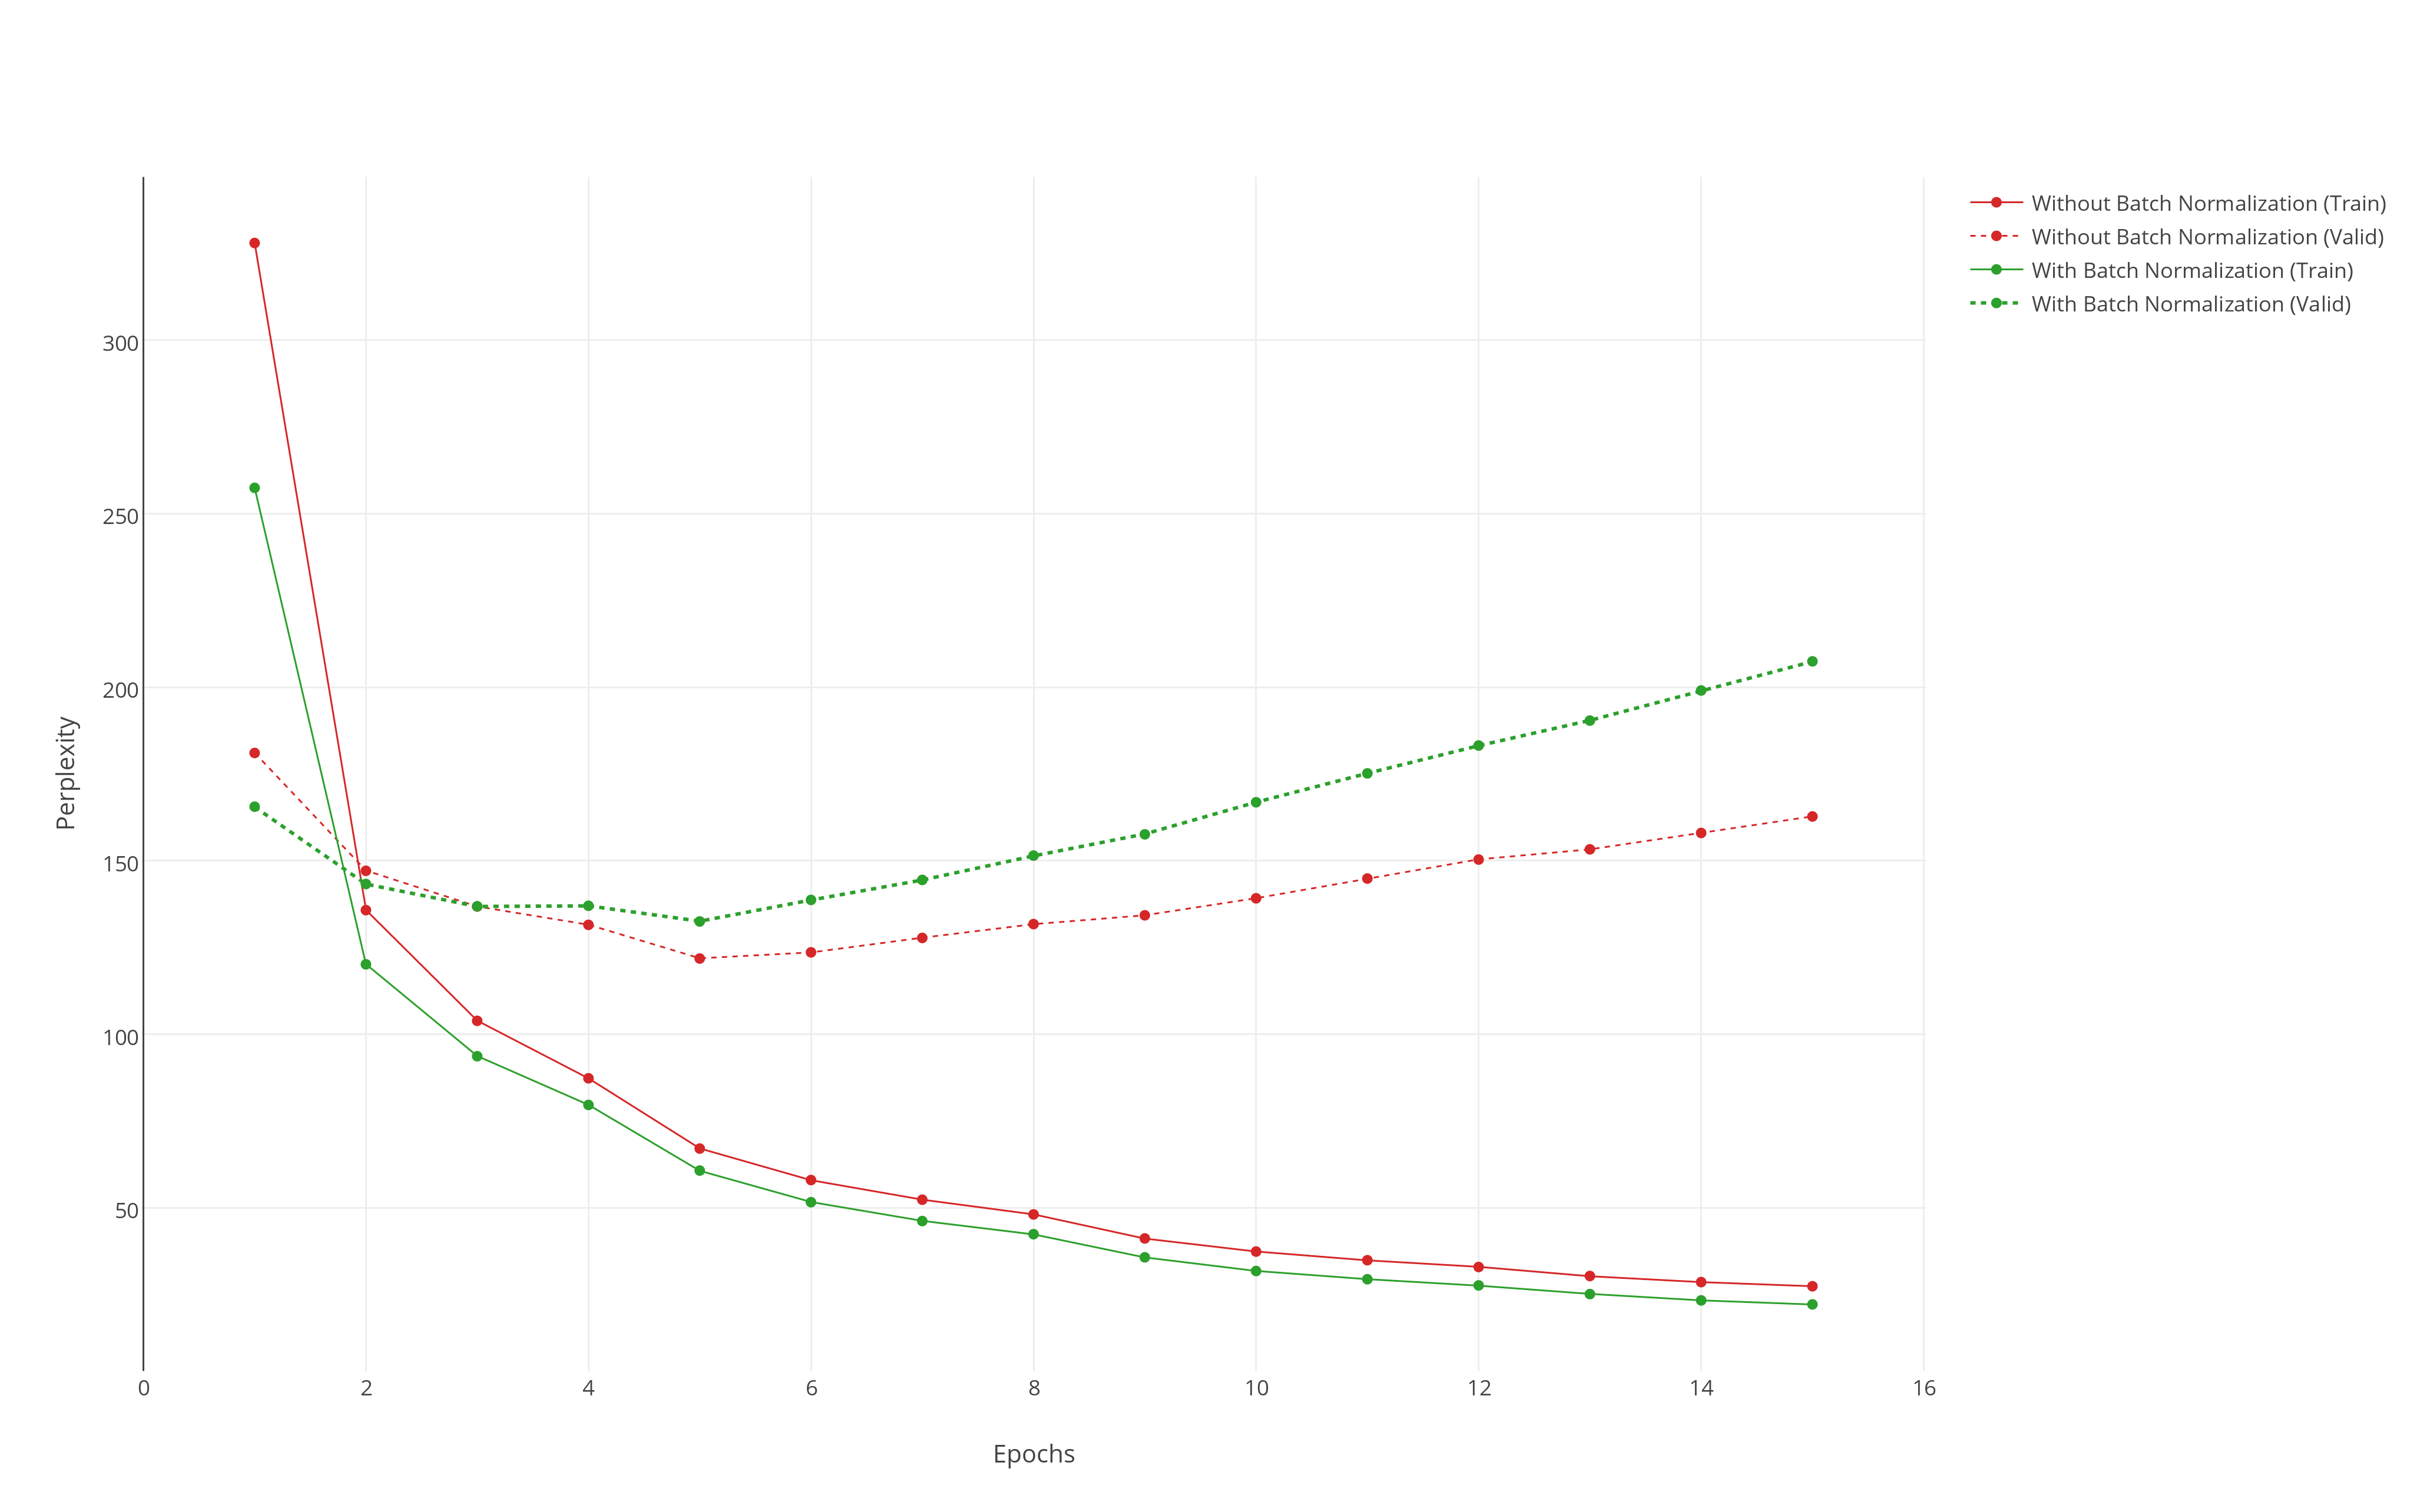
\includegraphics[width=100mm]{ptb_small_norm_plot.png}
  \caption{[Plot iterations instead of epochs, move legend to bottom and make font//lines larger] Small LSTM on Penn Treebank with and without batch normalization.}
  \label{overflow}
\end{figure}


{\renewcommand{\arraystretch}{1.4}

\begin{table}
	\begin{center}
		\begin{tabular}{lcr}
  			\hline
  			
			\multicolumn{1}{l}{\bf Model}  &\multicolumn{1}{c}{\bf Valid Set}  &\multicolumn{1}{c}{\bf Test Set} \\
  			
			\hline
  			
			\multicolumn{3}{c}{Penn Treebank} \\
  			
			\hline

  			Small LSTM		& 120.7 & 114.5 \\
  			Small LSTM (BN)	& 130.0 & 123.9 \\

  			\hline

  			Large LSTM		& 82.2 & \textbf{78.4} \\
  			Large LSTM (BN)	& \\

  			\hline

		\end{tabular}
	
		\caption{[\textit{Bold top and bottom lines}] Word-level perplexity on the Penn Treebank dataset.}

	\end{center}
\end{table}

\subsection{Speech Recognition}

\section{Discussion}

\section{Questions}
How do we normalize over time? [I can't do a reduction across time since I would be using the statistics of future words to predict past ones. Can you guys for speech or should we include a problem where we can normalize over time (e.g. sentiment)?]

Does batch normalization allow for a higher learning rate? [Table with learning rates and steps to convergence]

Shuffling data for language modeling? 


% References should be produced using the bibtex program from suitable
% BiBTeX files (here: strings, refs, manuals). The IEEEbib.bst bibliography
% style file from IEEE produces unsorted bibliography list.
% -------------------------------------------------------------------------
%\bibliographystyle{IEEEbib}

\bibliographystyle{natbib}
\bibliography{paperrefs}

\end{document}
